\title{DataStructure}


\documentclass[12pt]{article}
\usepackage{setspace}
\usepackage{import}
\usepackage{xifthen}
\usepackage{pdfpages}
\usepackage{transparent}
\usepackage{float}
\usepackage{tabularx,environ,amsmath,amssymb}
\usepackage{amsthm}
\usepackage[utf8]{inputenc}
\usepackage[english]{babel}

\newtheorem{theorem}{Theorem}[section]
\newtheorem{corollary}{Corollary}[theorem]
\newtheorem{lemma}[theorem]{Lemma}
\newtheorem*{example}{Example}

\newcommand{\vb}[1]{\verb|#1|}
\begin{document}
\maketitle


\section{AVL (Adelson - Velskii, Landis) Tree}

\begin{itemize}
  \item binary search
  \item the heights of the two child subtrees of any node differ by at most one.
\end{itemize}

ex)

\begin{figure}[H]
	\centering
	\def\svgwidth{\columnwidth}
	\import{./figures/}{avl.pdf_tex}
	\caption{Example of AVL : from any node, left and right tree has height different at most 1.}
	\label{fig:avl}
\end{figure}

* Insertion (a,b,e)

Single Rotation :

\begin{figure}[H]
	\centering
	\def\svgwidth{\columnwidth}
	\import{./figures/}{sr.pdf_tex}
	\caption{single rotation on a,b,e}
	\label{fig:sr}
\end{figure}

Double Rotation:
\begin{figure}[H]
	\centering
	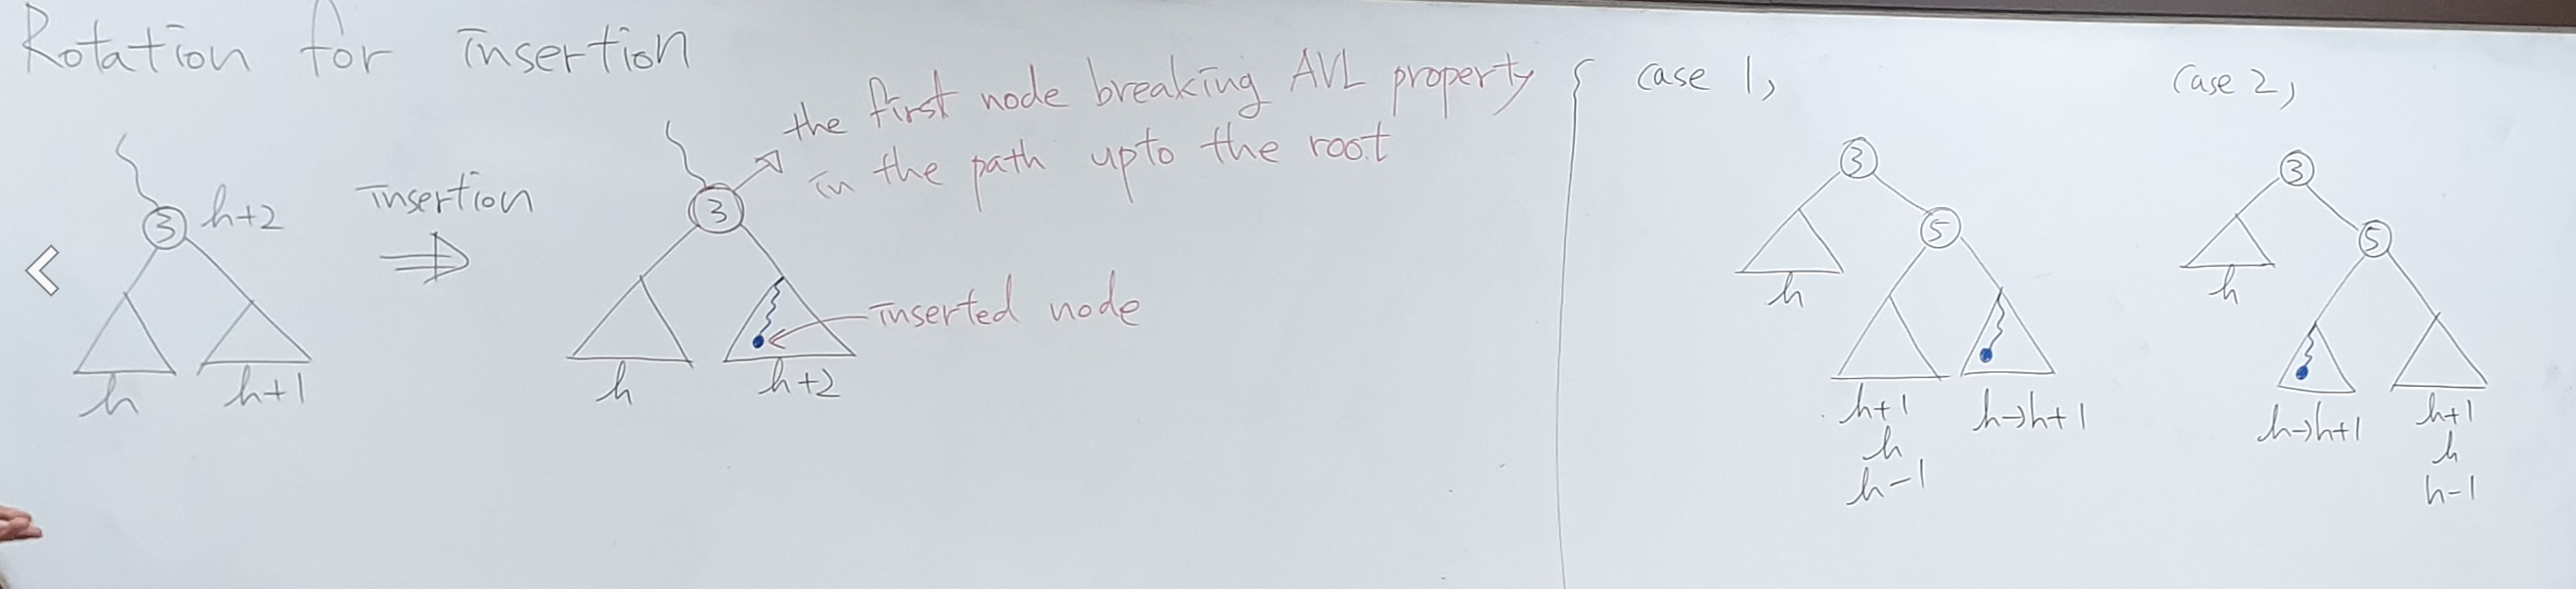
\includegraphics[width=0.95\textwidth]{img/doublerot.png}
	\caption{}
	\label{}
\end{figure}


Rotation for insertion:

\begin{figure}[H]
	\centering
	\def\svgwidth{\columnwidth}
	\import{./figures/}{dr.pdf_tex}
	\caption{Double rotation on c,d}
	\label{fig:dr}
\end{figure}

If h + 1, 3 should be h+3 before insertion.
If h-1, 5 should be the first node breaking AVL property after insertion.



\end{document}
